\subsection{Mismatched Crowdsourcing}
\label{sec:MC}

%\begin{figure}
%  \centerline{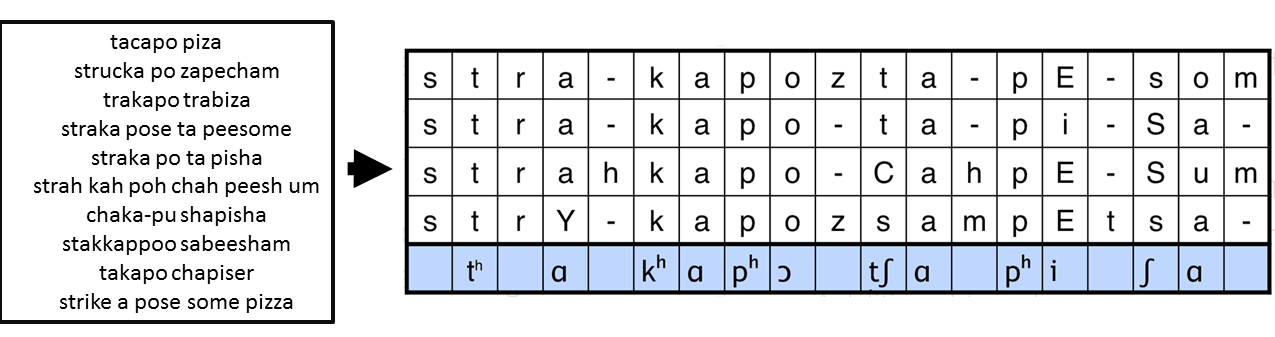
\includegraphics[width=5in]{../figs/fig_jyothi.png}}
%  \caption{In mismatched crowdsourcing, people who don't speak a
%    language (in this case Swahili) are asked to transcribe it using
%    nonsense syllables in the orthography of their own language (in
%    this case English).  There is a great deal of variability in their
%    responses (left), but information about the phonetic content of
%    the speech can be derived by merging the transcripts (top four
%    rows at right) and decoding using a model of non-native speech
%    perception (decoding result in the bottom row at right).}
%  \label{fig:mc}
%\end{figure}
%% comments: it's odd that all four of the illustrated transcripts begin
%% with the sequence [str], but the decoded result does not include the
%% [s] or the [r]. Perhaps it would be better to choose four transcripts
%% that vary more widely (and even indicate which orthographic strings
%% they correspond to) so that the derived result looks more plausible.
%% It is also odd that the formation of lambda involves choosing 5 best
%% MTs, but the figure shows 4 MTs.
%% Also, it is odd that pseudo-phonetic code is used in the transcripts
%% instead of IPA; IPA only occurs in the decoded result. Is there a
%% compelling reason for that?  Also, this figure is an excellent
%% candidate for vector graphic format rather than raster, since it's
%% all lines and text. I'm happy to help out with recreating figures in
%% vector format if that's desired.
%% Finally, I think this figure belongs after the following paragraph,
%% which could sensibly be merged into the opening paragraph of this
%% section. 

The second set of PTs were computed by sending audio in the target
language to non-speakers of the target language (all transcribers were
speakers of American English, and the plurality were monolingual), and
asking them to write what they hear.  Denote using $T$ the set of text
transcripts produced by these English-speaking crowd workers.
Mismatched transcripts must be converted into the form of a pmf over
target-language phone sequences, $\pi(\phi^\ell|T)$.  As an
intermediate step towards this goal, prior work~\cite{JHJ15b}
developed techniques to merge the transcripts in $T$ into a
distribution $\rho(\lambda|T)$ over representative crowd-worker
transcripts, denoted $\lambda$.  The representative transcripts,
$\lambda$, use the same orthography as the crowd worker transcripts
$T$ (English nonsense syllables), but differ in reliability, as
follows.  Formation of $\lambda$ from $T$ involves data filtering
(choosing the most representative 5 transcripts out of each set of 10,
using pair-wise string edit distances among the transcripts),
conversion of annotation-language orthography into a pseudo-phonetic
code in order to represent common letter sequences (e.g., ``ee'' in
English orthography represents the phoneme \ipa{/i/}), and a weighted
voting scheme in which the weight of each transcript is proportional
to the frequency with which it matches the other transcripts.

%% Unclear point (maybe just to me): What exactly is lambda? In the
%% previous paragraph it's described as the set of representative
%% transcriptions, whereas in the next paragraph it is described as a
%% confusion network, and in a later paragraph seems to be used to refer
%% to (the set of) "graphemes in the annotation language".
Once transcripts have been aligned and filtered to create the
orthographic confusion network $\rho(\lambda|T)$, they are then
translated into a distribution over phonemic transcriptions according
to:
\begin{align}
  \rho(\phi|T) &=
  \sum_{\lambda} \rho(\phi|\lambda,T) \rho(\lambda|T) \notag \\
  &\approx \max_{\lambda}  \rho(\phi|\lambda) \rho(\lambda|T) \notag \\
  &= \max_{\lambda}  \left(\frac{\rho(\lambda|\phi)}{\rho(\lambda)}
  \rho(\phi)\right) \rho(\lambda|T) 
\label{eq:PT}
\end{align}

The terms other than $\rho(\lambda|T)$ in Equation~(\ref{eq:PT}) are
estimated as follows.  $\rho(\lambda)$ is modeled using a simple
context-free prior over the letter sequences in $\lambda$.
$\rho(\phi)$ is modeled using a bigram phone language model, trained
on a corpus of Wikipedia text in the target language, converted into
phone sequences as described in Section~\ref{sec:trainwithlm}.
$\rho(\lambda|\phi)$ is called the misperception G2P, as it maps to
graphemes in the annotation language, $\lambda$, from phones in the
utterance language, $\phi$.  This section describes methods that 
estimate $\rho(\lambda|\phi)$ directly; Section~\ref{sec:eegchanmod} 
describes methods that decompose $\rho(\lambda|\phi)$ 
into separate misperception and G2P transducers.
%% shouldn't it be called "misperception P2G" instead of G2P?

The misperception G2P ($\rho(\lambda|\phi)$) can be trained directly
using the Carmel toolkit \cite{Knight99} as an FST mapping phones to
letters based on representative transcripts $\lambda$ (and their
corresponding native transcripts) for speech {\em in languages other
  than the target language}. We assume that misperceptions depend more
heavily on the annotation language than on the utterance language, and
that therefore a model $\rho(\lambda|\phi)$ trained using a universal
phone set for $\phi$ is also a good model of $\rho(\lambda|\phi)$ for
the target language. Note that, while this assumption is not entirely
accurate, it is necessitated by the requirement that no native
transcriptions in the target language can be used in building any part
of our system.
%We also allow this FST to delete phones and insert letters.

